\section{Optimization Approximation}

Consider the program of minimizing a function $f: X \to \mathbb{R}$. In many scenarios, it is hard to find an optimal or it is hard to compute the value of $f(x)$. Isaac Vandermeulen, Roderich Groß, Andreas Kolling \cite{vandermeulen2019balanced} has introduced a method that find a function $f_1: X \to \mathbb{R}$ such that $f(x) = c(f_1(x)) + v$ where $c$ is a monotonically increasing function and $v$ is a random variable. 

Let some bounds on $v$ as follows: $\alpha$ $\in$ (0, 0.5) and $b_\alpha^-$, $b_\alpha^+$ $\in$ $\mathbb{R}_+$

\[
\mathbb{P}[-b_\alpha^- \leq v] = \mathbb{P}[v \leq +b_\alpha^+] = 1 - \alpha
\]

Let $x^*$ and $x^*_1$ be the optimal values for $f$ and $f_1$.

\[
(A): f(x^*_1) \leq f(x^*) + b_\alpha^- + b_\alpha^+
\]

\begin{theorem}[Approximation]:
\[
\mathbb{P}[A] \geq (1 - \alpha)^2
\]
\end{theorem}

The theorem states that if one can find $f_1$ with small variance on $v$, minimizing $f_1$ provides a good solution on $f$ with high probability.

\begin{figure}[h!]
\centering
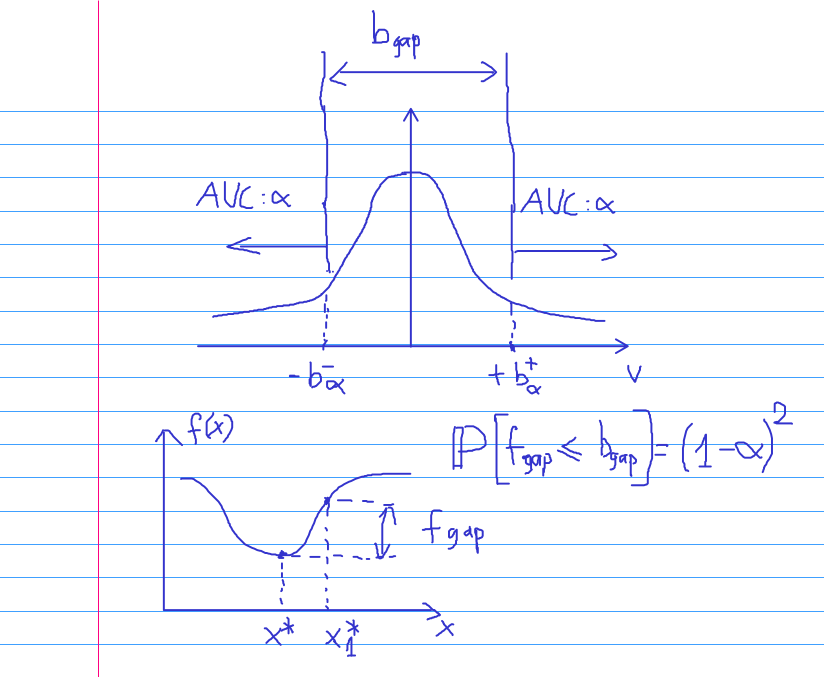
\includegraphics[width=0.8\textwidth]{assets/optimization.png}
\caption{Optimization}
\label{fig:optimization}
\end{figure}





In \cite{vandermeulen2019balanced}, the authors defined average cycle length as follow:

\begin{definition}[Average cycle length]
\[
C_a^{(k)} = \frac{\sum_{i \in V_k} \sum_{j \in V_k} A_{ij}}{|V_k| - 1}
\]
\end{definition}

Where $V_k$ is the set of nodes in the partition $k$.

By choosing $f_1$ as maximum average cycle length, the authors approximated the solution of problem \ref{prob:problem3} by minimizing:

\[
O_0 = max\{C_a^{(k)}\}_{k=1}^{K}
\]

However, maximum average cycle length does not contain any information about the other $K-1$ smaller cycles. We have experimented with different $f_1$ objective functions.


\begin{figure}[h!]
\centering
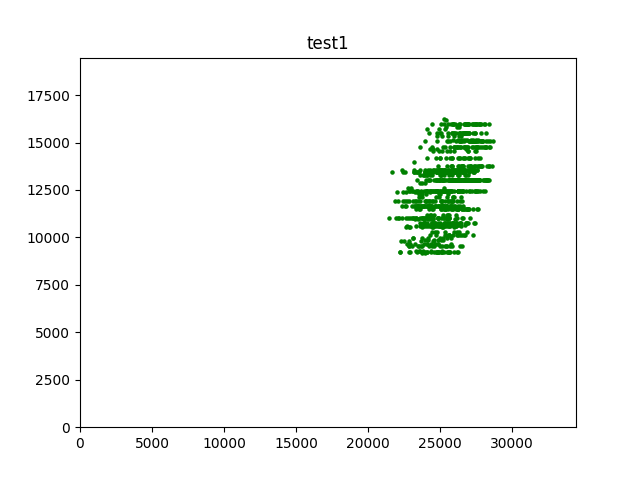
\includegraphics[width=0.8\textwidth]{assets/test1max.png}
\caption{maximum tsp cycle length over test1 objective of all 5-partitions in a 15 nodes network}
\label{fig:test1max}
\end{figure}

\begin{figure}[h!]
\centering
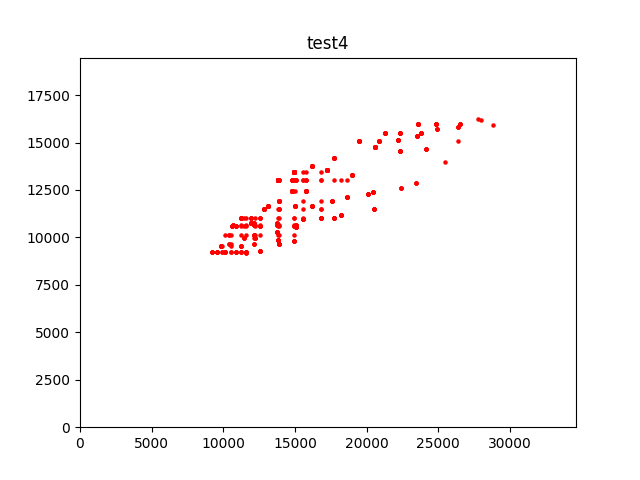
\includegraphics[width=0.8\textwidth]{assets/test4max.png}
\caption{maximum tsp cycle length over test4 objective of all 5-partitions in a 15 nodes network}
\label{fig:test4max}
\end{figure}

\begin{figure}[h!]
\centering
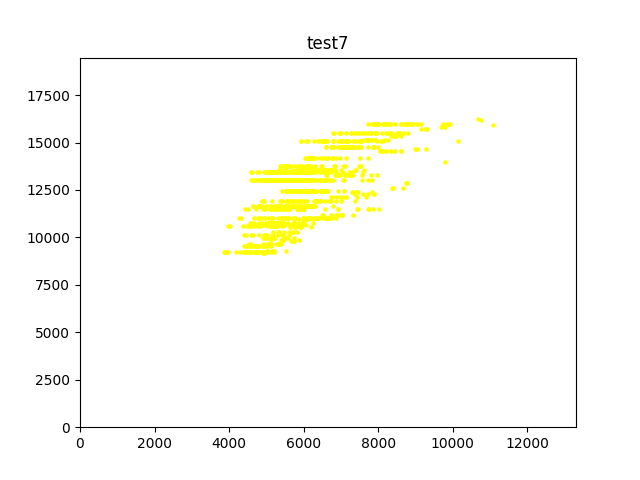
\includegraphics[width=0.8\textwidth]{assets/test7max.png}
\caption{maximum tsp cycle length over test7 objective of all 5-partitions in a 15 nodes network}
\label{fig:test7max}
\end{figure}

\begin{figure}[h!]
\centering
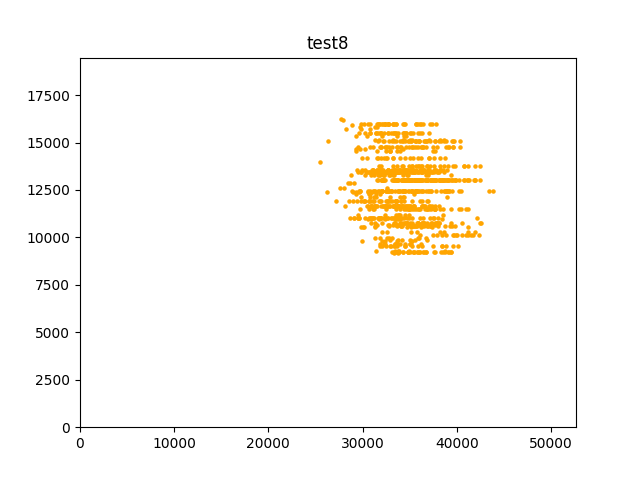
\includegraphics[width=0.8\textwidth]{assets/test8max.png}
\caption{maximum tsp cycle length over test8 objective of all 5-partitions in a 15 nodes network}
\label{fig:test8max}
\end{figure}



\begin{figure}[h!]
\centering
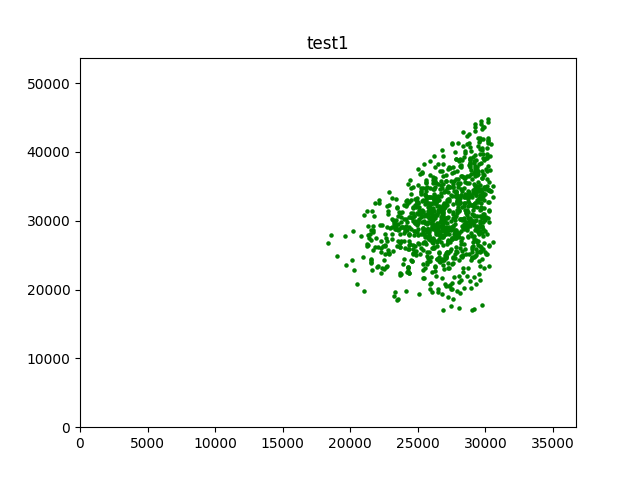
\includegraphics[width=0.8\textwidth]{assets/test1sum.png}
\caption{sum tsp cycle length over test1 objective of all 5-partitions in a 15 nodes network}
\label{fig:test1sum}
\end{figure}

\begin{figure}[h!]
\centering
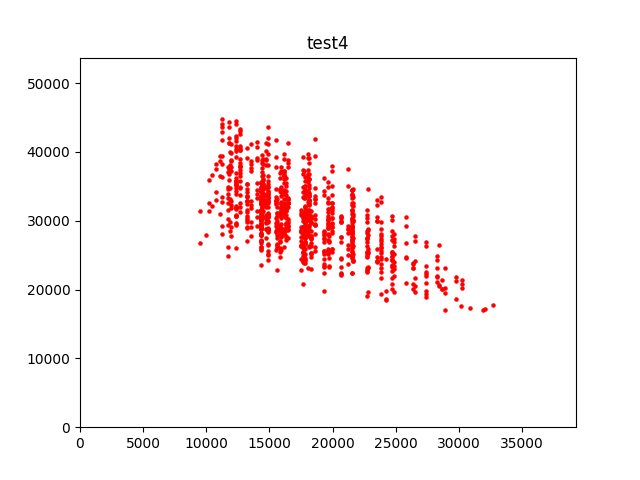
\includegraphics[width=0.8\textwidth]{assets/test4sum.png}
\caption{sum tsp cycle length over test4 objective of all 5-partitions in a 15 nodes network}
\label{fig:test4sum}
\end{figure}

\begin{figure}[h!]
\centering
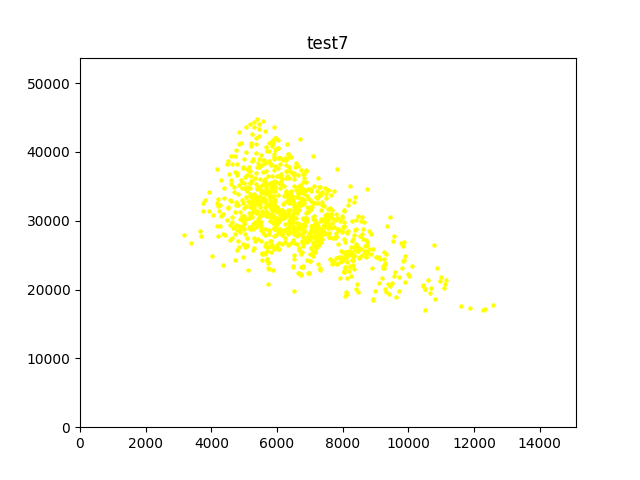
\includegraphics[width=0.8\textwidth]{assets/test7sum.png}
\caption{sum tsp cycle length over test7 objective of all 5-partitions in a 15 nodes network}
\label{fig:test7sum}
\end{figure}

\begin{figure}[h!]
\centering
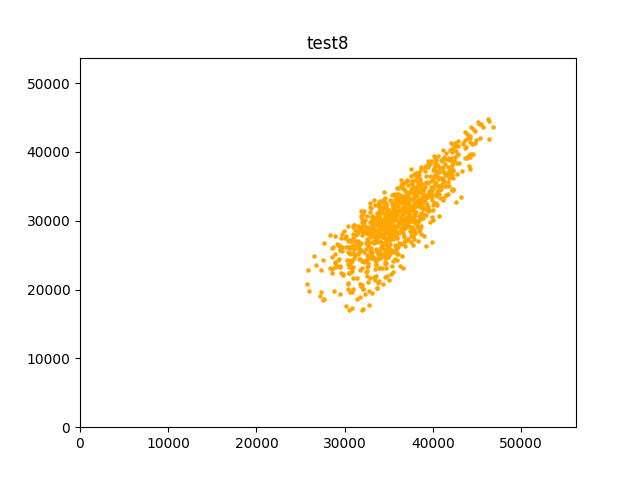
\includegraphics[width=0.8\textwidth]{assets/test8sum.png}
\caption{sum tsp cycle length over test8 objective of all 5-partitions in a 15 nodes network}
\label{fig:test8sum}
\end{figure}

From the pattern on each $f_1$ function to the $f$, we can predict that test4 and test7 tend to provide a smaller maximum cycle length and test1 and test 8 tend to provide a smaller total cycle length.
